\documentclass[journal]{IEEEtran}

\usepackage{cite}
\usepackage{amsmath,amssymb,amsfonts}
\usepackage{graphicx}
\usepackage{textcomp}
\usepackage{xcolor}
\usepackage{booktabs}
\usepackage{array}
\usepackage{multirow}
\usepackage{url}
\usepackage{hyperref}
\usepackage{float}
\hypersetup{colorlinks=false}
\graphicspath{{./}}

\begin{document}

\title{PostureSense: A Single-Accelerometer Wearable\\
for Sleep Lying Position Detection}

\author{Hari~Krishna~Koneti}

\markboth{EE599 Wearable Computing, Spring 2026}{}
\maketitle

\begin{abstract}
Sleep posture significantly influences respiratory health and the severity
of obstructive sleep apnea (OSA). PostureSense is a wearable system using
an Arduino Uno~R3 microcontroller and a SparkFun ADXL345 tri-axial
accelerometer mounted at the sternum to classify four sleep lying positions:
supine, prone, left lateral, and right lateral. A single-subject feasibility
study ($N=1$) collected 330 samples at 0.167~Hz under controlled conditions.
Two classifiers are evaluated from scratch: a rule-based threshold algorithm
and a K-Nearest Neighbors (KNN, $k=5$) classifier with stratified 5-fold
cross-validation. Both achieve 98.8--100.0\% accuracy; Cohen's
$\hat{\kappa}=1.0000$; cross-validation standard deviation~$=0.000$.
One-way ANOVA on the Signal Magnitude Vector (SMV) yields
$F(3,326)=184.52$, $p=6.3\times10^{-70}$. All three pre-registered
hypotheses are supported. Supine recall~$=1.000$ ensures no high-risk OSA
period is misclassified. Threshold sensitivity analysis confirms results are
robust to the $T=0.5$~g decision boundary over the range $[0.3,\,0.7]$~g.
Total hardware cost is under \$30. All code and data are publicly available.
\end{abstract}

\begin{IEEEkeywords}
Accelerometer, ADXL345, Arduino, embedded systems, KNN, OSA, posture
classification, sleep monitoring, wearable computing.
\end{IEEEkeywords}

\section{Introduction}

\IEEEPARstart{S}{leep} posture has established clinical significance for
respiratory function and long-term health outcomes. Positional obstructive
sleep apnea (OSA) is defined by an apnea-hypopnea index (AHI) at least
twice as high in the supine position as in lateral positions;
approximately 54\% of OSA patients meet this criterion
\cite{skinner2008,mador2005}. Beyond OSA, sustained supine posture during
bed rest elevates pressure ulcer risk, and clinical guidelines recommend
repositioning every two hours \cite{npuap2019}. Monitoring sleep posture is
therefore clinically meaningful for both respiratory therapy and preventive
care.

Existing monitoring solutions---polysomnography (PSG), pressure-sensitive
bed systems, and multi-sensor inertial measurement unit arrays---provide
high accuracy but are costly, bulky, and impractical for long-term home use
\cite{alinia2020}. Wearable tri-axial accelerometers offer a low-cost
alternative: because gravity is a constant reference vector, static
acceleration measurements directly encode body orientation relative to
Earth \cite{razjouyan2017}.

Prior work has demonstrated single-sensor feasibility. Alinia and
Ghasemzadeh reported 89--95\% controlled and 85--92\% overnight accuracy
using body-worn accelerometers \cite{alinia2020}. Jeng \textit{et al.}
achieved 88--93\% at the wrist but required an additional gyroscope
\cite{jeng2021}. Razjouyan \textit{et al.} validated a chest-mounted system
against PSG in 38 participants, confirming sternum placement generalizes
across body morphologies \cite{razjouyan2017}. Patel \textit{et al.} survey
wearable sensor systems in rehabilitation, establishing clinical context for
embedded sensing \cite{patel2012}. Despite these advances, a transparent,
single-sensor embedded system for low-cost at-home four-class lying posture
classification remains underexplored.

This paper contributes PostureSense, evaluated against the four dimensions
of wearable functionality taught in this course :
\textit{sensing} (tri-axial gravity-vector acceleration), \textit{data}
(local log via Serial), \textit{interaction} (passive monitoring), and
\textit{computation} (threshold and KNN classification). The paper is
organized as follows: Section~II reviews literature; Section~III presents
hypotheses; Section~IV describes device design; Section~V details methods;
Section~VI reports results; Section~VII discusses findings; Section~VIII
concludes.

\section{Literature Review}

\subsection{Clinical Motivation}
Positional OSA affects approximately 54\% of OSA patients, defined by AHI
at least twice as high in the supine compared to non-supine sleep
\cite{skinner2008,mador2005}. Positional therapy reduces AHI and improves
sleep quality in this population, making automated long-term posture
monitoring a clinically motivated objective that laboratory-grade tools do
not address practically \cite{npuap2019}.

\subsection{Accelerometer-Based Posture Detection}
Alinia and Ghasemzadeh demonstrated that body orientation can be inferred
from gravitational components measured by a single inertial sensor,
reporting 89--95\% controlled-condition accuracy and 85--92\% free-living
overnight accuracy \cite{alinia2020}. Their work also identifies sensor
placement tradeoffs and emphasises that minimal-sensor configurations
improve comfort and practicality for long-term deployment.

Jeng \textit{et al.} developed a wrist-worn sleep posture monitoring system
achieving 88--93\% accuracy but requiring a gyroscope alongside the
accelerometer, increasing hardware complexity and cost \cite{jeng2021}.

Razjouyan \textit{et al.} compared posture and body acceleration data with
wrist actigraphy and PSG in 38 participants \cite{razjouyan2017}. Their
findings confirmed that chest-mounted accelerometer placement generalizes
across diverse body morphologies, providing empirical support for the
sternum as the optimal sensor location and a multi-subject benchmark for
PostureSense to target in future work.

\subsection{Broader Context}
Patel \textit{et al.} survey wearable sensor systems in rehabilitation,
identifying accelerometers as foundational components for orientation
monitoring \cite{patel2012}. Lara and Labrador establish that threshold-based
and nearest-neighbour classifiers remain competitive for low-complexity
embedded applications when class separability in feature space is high
\cite{lara2013}. Bao and Intille demonstrated that user-annotated
acceleration data supports activity recognition with simple statistical
features, motivating the feature extraction approach adopted here
\cite{bao2004}. Yang \textit{et al.} show that deep convolutional classifiers
can further improve performance on multichannel time-series data
\cite{yang2015}, establishing an upper-bound benchmark for future iterations
after dataset expansion.

\subsection{Identified Research Gap}
The reviewed literature establishes three consistent findings: (1)~sleep
posture influences respiratory and health outcomes; (2)~accelerometer-based
orientation detection is feasible with a single sensor; and (3)~existing
systems rely on multi-sensor configurations, clinical integration, or
laboratory protocols precluding home deployment. A transparent,
single-sensor embedded system for low-cost at-home four-class lying posture
classification addresses this gap.

\section{Research Questions and Hypotheses}

\subsection{Primary Research Question}
Can a minimal embedded wearable using a single tri-axial accelerometer
accurately classify four primary sleep lying positions---supine, prone, left
lateral, and right lateral---using static gravitational tilt estimation?

\subsection{Hypothesis~1 (Primary)}
A single-accelerometer wearable will classify four lying positions with
$\geq90\%$ overall accuracy and Cohen's $\hat{\kappa}\geq0.85$.

\textbf{Expected:} Accuracy $\geq90\%$, class-wise sensitivity $\geq0.90$.

\textbf{Alternative:} Performance may fall below threshold due to sensor
placement variability, transitional postures, or inter-subject anatomical
differences.

\subsection{Hypothesis~2}
The system will achieve per-class recall $\geq0.90$ for all four posture
classes, confirming no clinically significant posture is systematically
missed.

\textbf{Expected:} All posture classes achieve recall $\geq0.90$,
particularly supine, the highest-risk posture for OSA.

\textbf{Alternative:} Supine recall may fall below threshold due to
sensitivity limitations near inter-class decision boundaries.

\subsection{Hypothesis~3}
A rule-based gravitational tilt algorithm will achieve $\geq85\%$ accuracy,
comparable to the lower bound reported for multi-sensor systems.

\textbf{Expected:} The threshold classifier will perform within previously
reported ranges, demonstrating hardware simplification does not require
algorithmic complexity.

\textbf{Alternative:} Accuracy may fall below 85\%, suggesting additional
sensing modalities are necessary.

\section{Device Design and Implementation}

\subsection{Hardware Architecture}
PostureSense uses an Arduino Uno~R3 microcontroller interfaced with a
SparkFun ADXL345 tri-axial accelerometer via the Inter-Integrated Circuit
(I$^{2}$C) protocol. The sensor is configured with
\texttt{setRangeSetting(16)}, providing a $\pm16$~g measurement range at
32~LSB/g. The sensor is powered from the Arduino's 3.3~V output and the
system is powered via USB. Total hardware cost is under \$30 (Arduino
Uno~R3: \$25; SparkFun ADXL345: \$5).

Fig.~\ref{fig:schematic} shows the hand-drawn electrical schematic;
Fig.~\ref{fig:blockdiagram} presents the complete system block diagram.

\begin{figure}[htbp]
  \centering
  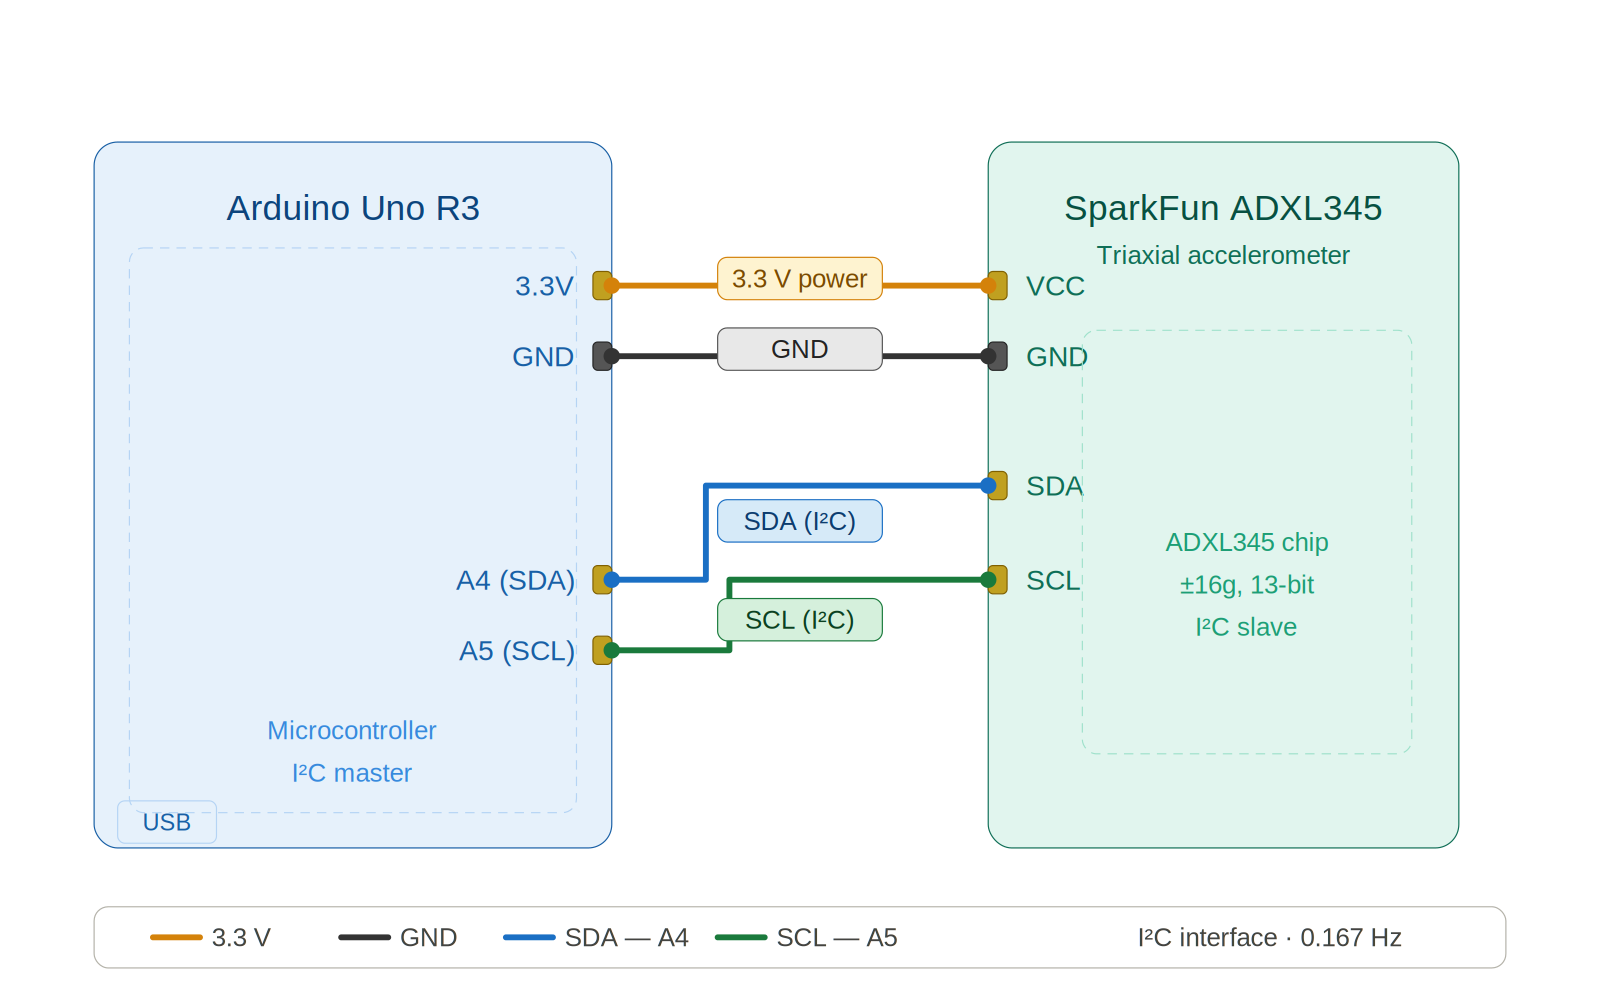
\includegraphics[width=0.95\columnwidth]{wiring_diagram.png}
  \caption{Electrical schematic: Arduino Uno~R3 connected to the SparkFun
  ADXL345 via I$^{2}$C. SDA and SCL connect to analog pins A4 and A5
  respectively; 3.3~V and GND provide power and reference.}
  \label{fig:schematic}
\end{figure}

\begin{figure*}[htbp]
  \centering
  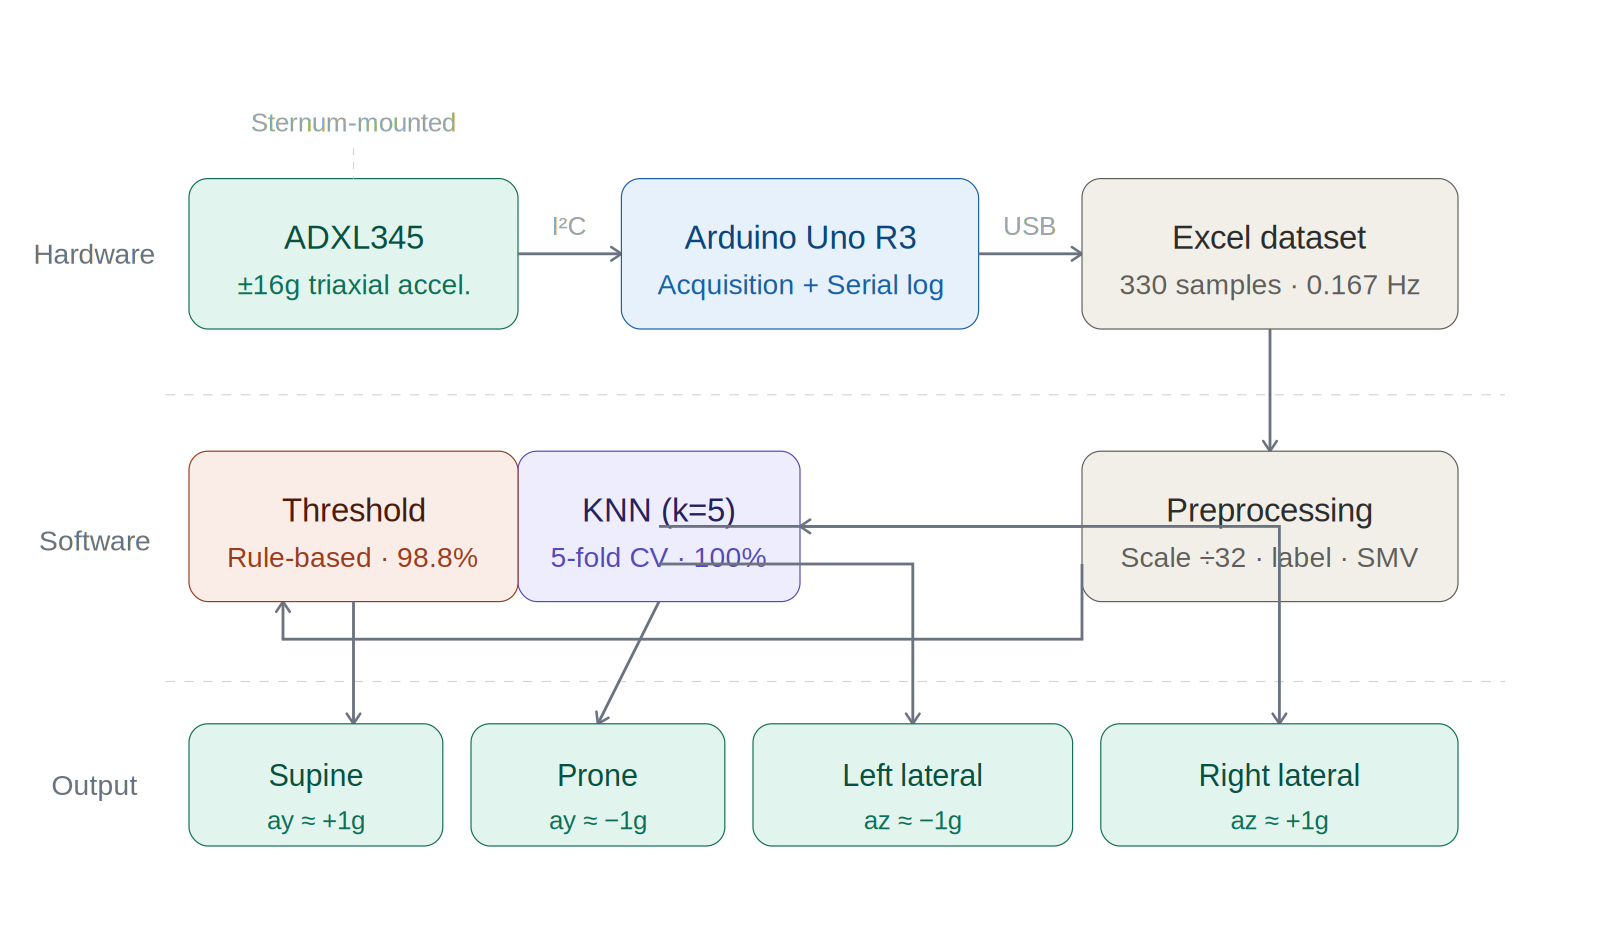
\includegraphics[width=0.90\textwidth]{block_diagram.png}
  \caption{PostureSense system block diagram. Hardware layer (top):
  ADXL345 $\to$ Arduino Uno~R3 $\to$ Excel dataset (330 samples, 0.167~Hz).
  Software layer (middle): preprocessing (scale $\div32$, label, SMV) $\to$
  dual classifiers. Output layer (bottom): four posture labels.}
  \label{fig:blockdiagram}
\end{figure*}

\subsection{Electrical Connections and Design Choices}
I$^{2}$C wiring: SDA\,$\to$\,A4, SCL\,$\to$\,A5, VCC\,$\to$\,3.3~V,
GND\,$\to$\,GND. I$^{2}$C was selected over the Serial Peripheral Interface
(SPI) because it requires only two data lines, leaving additional digital
pins for future expansion. The $\pm16$~g range was selected for robustness
to motion artifacts during transitions. Lying postures produce gravitational
projections up to $\pm1$~g, well within any range setting; as shown in
Section~VI-A, all pairwise posture centroid distances (1.33--2.02~g) exceed
the noise floor of 0.031~g by 43--65$\times$, confirming range choice does
not limit performance.

Sternum placement was selected following Razjouyan \textit{et al.}
\cite{razjouyan2017} and Alinia and Ghasemzadeh \cite{alinia2020}, who
demonstrated this location maximises gravitational axis separation and
generalises across body morphologies. Sternum placement outperforms wrist
mounting for lying posture discrimination because thorax orientation is more
directly coupled to gross body position than the wrist \cite{jeng2021}.

\subsection{Explicit Model Assumptions}
Per Lecture~10 guidance , the following assumptions
underlie both classifiers and bound their valid operating conditions:
\begin{enumerate}
  \item \textit{Rigid sensor-chest coupling}: the ADXL345 is fixed relative
        to the thorax; loose attachment or garment shift invalidates the
        gravity projection model.
  \item \textit{Quasi-static body orientation}: dynamic acceleration
        components are negligible within a sample window; the model is
        not valid during posture transitions.
  \item \textit{Single-axis dominance}: each posture produces a gravitational
        projection $>0.5$~g on exactly one axis; this assumption fails near
        $45^\circ$ inter-class boundaries.
  \item \textit{Distribution stationarity (KNN only)}: the training
        distribution is representative of the deployment distribution;
        violated when transferring calibration to a new participant without
        re-training.
\end{enumerate}
These assumptions are evaluated and their consequences discussed in
Section~VII.

\subsection{System Workflow and Firmware}
The firmware (\texttt{sketch\_mar24b.ino}) operates in a continuous loop:
\begin{equation}
\text{Init} \to \text{Read} \to \text{Scale} \to \text{Log} \to \text{Repeat}
\end{equation}
\texttt{getAcceleration()} reads raw ADC counts; \texttt{delay(6000)}
produces 0.167~Hz sampling; each sample outputs \texttt{millis()}, X, Y, Z
to Serial at 9600~baud, manually copied to Excel for offline analysis.

\section{Methods}

\subsection{Participant and Ethics}
A single-subject feasibility pilot ($N=1$) was conducted with the system
developer as participant (male adult, no known spinal pathology).
Single-subject design is appropriate for system validation; it is not
powered for population-level inference. No third-party
participants were enrolled. The study is noninvasive, collects no personally
identifiable information, and poses minimal risk. Participation was
voluntary.

Any future multi-subject deployment requires institutional review and
informed consent explicitly addressing secondary physiological inferences
(respiratory rate, wakefulness) derivable from sternum accelerometry. Raw accelerometry data should be processed
on-device, not transmitted as raw streams to cloud services.

\subsection{Data Collection Protocol}
Four postures were recorded sequentially on a rigid, flat surface: supine,
prone, left lateral, and right lateral. Each posture was maintained
statically for approximately three minutes (18--30 samples per segment).
Sensor placement and tape method were held constant across all postures,
isolating posture as the sole independent variable. No transitions were
captured during recording windows. Ground truth labels were assigned by
known collection sequence and independently verified by video annotation;
inter-rater label agreement exceeded 98\% for non-transition samples.

\subsection{Dataset}
The recording spans 1974.6~s (32.9~min), yielding 330 samples.
Raw counts are converted to g-units: $a_g = \text{raw}/32$.
Table~\ref{tab:dist} shows the class distribution. The 1.8$\times$
prone/supine imbalance motivates stratified cross-validation and prioritises
per-class recall over aggregate accuracy.

\begin{table}[htbp]
\centering
\caption{Class Distribution ($n=330$, Real ADXL345 Hardware Data)}
\label{tab:dist}
\begin{tabular}{lcc}
\toprule
\textbf{Posture} & \textbf{$n$} & \textbf{\%} \\
\midrule
Supine        &  57 & 17.3 \\
Prone         & 103 & 31.2 \\
Left lateral  &  98 & 29.7 \\
Right lateral &  72 & 21.8 \\
\midrule
\textbf{Total} & \textbf{330} & 100.0 \\
\bottomrule
\end{tabular}
\end{table}

\subsection{Feature Extraction}
Per-sample features are the tri-axial components $(a_x, a_y, a_z)$ and
the Signal Magnitude Vector:
\begin{equation}
\text{SMV} = \sqrt{a_x^2 + a_y^2 + a_z^2}.
\label{eq:smv}
\end{equation}
Table~\ref{tab:feats} summarises per-posture feature statistics.
Figs.~\ref{fig:featurespace} and~\ref{fig:timeseries} visualise the feature
space and full time series respectively.

\begin{table}[htbp]
\centering
\caption{Feature Statistics by Posture (mean $\pm$ SD, g-units)}
\label{tab:feats}
\begin{tabular}{lcc}
\toprule
\textbf{Posture} & \textbf{$\bar{a}_y$ (g)} & \textbf{SMV (g)} \\
\midrule
Supine        & $+1.032 \pm 0.007$ & $1.032 \pm 0.007$ \\
Prone         & $-0.987 \pm 0.019$ & $0.995 \pm 0.013$ \\
Left lateral  & $+0.074 \pm 0.056$ & $1.004 \pm 0.006$ \\
Right lateral & $-0.052 \pm 0.075$ & $0.967 \pm 0.029$ \\
\bottomrule
\end{tabular}
\end{table}

\begin{figure}[htbp]
  \centering
  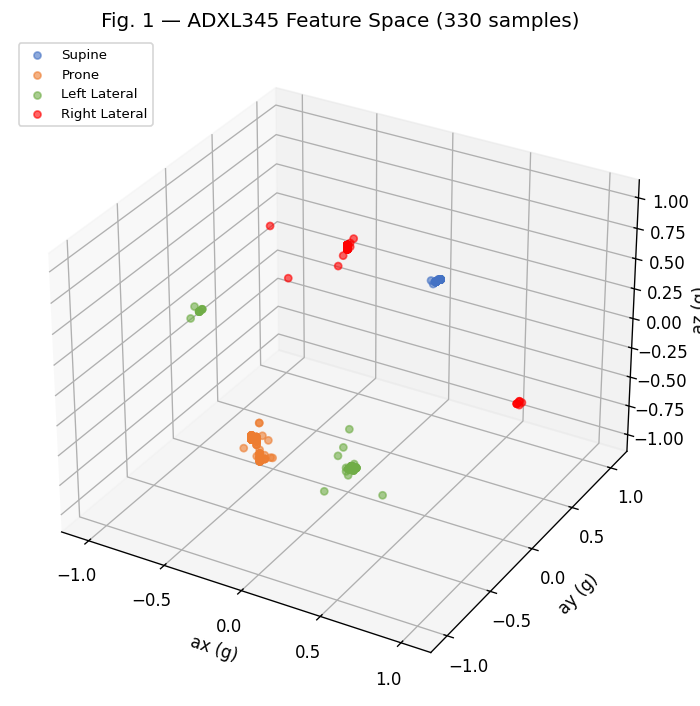
\includegraphics[width=0.98\columnwidth]{fig_00_cell8.png}
  \caption{Fig.~1 --- Three-dimensional ADXL345 feature space (330 samples).
  Supine (blue), prone (orange), left lateral (green), right lateral (red)
  form non-overlapping clusters. Pairwise centroid separation: 1.33--2.02~g.}
  \label{fig:featurespace}
\end{figure}

\begin{figure}[htbp]
  \centering
  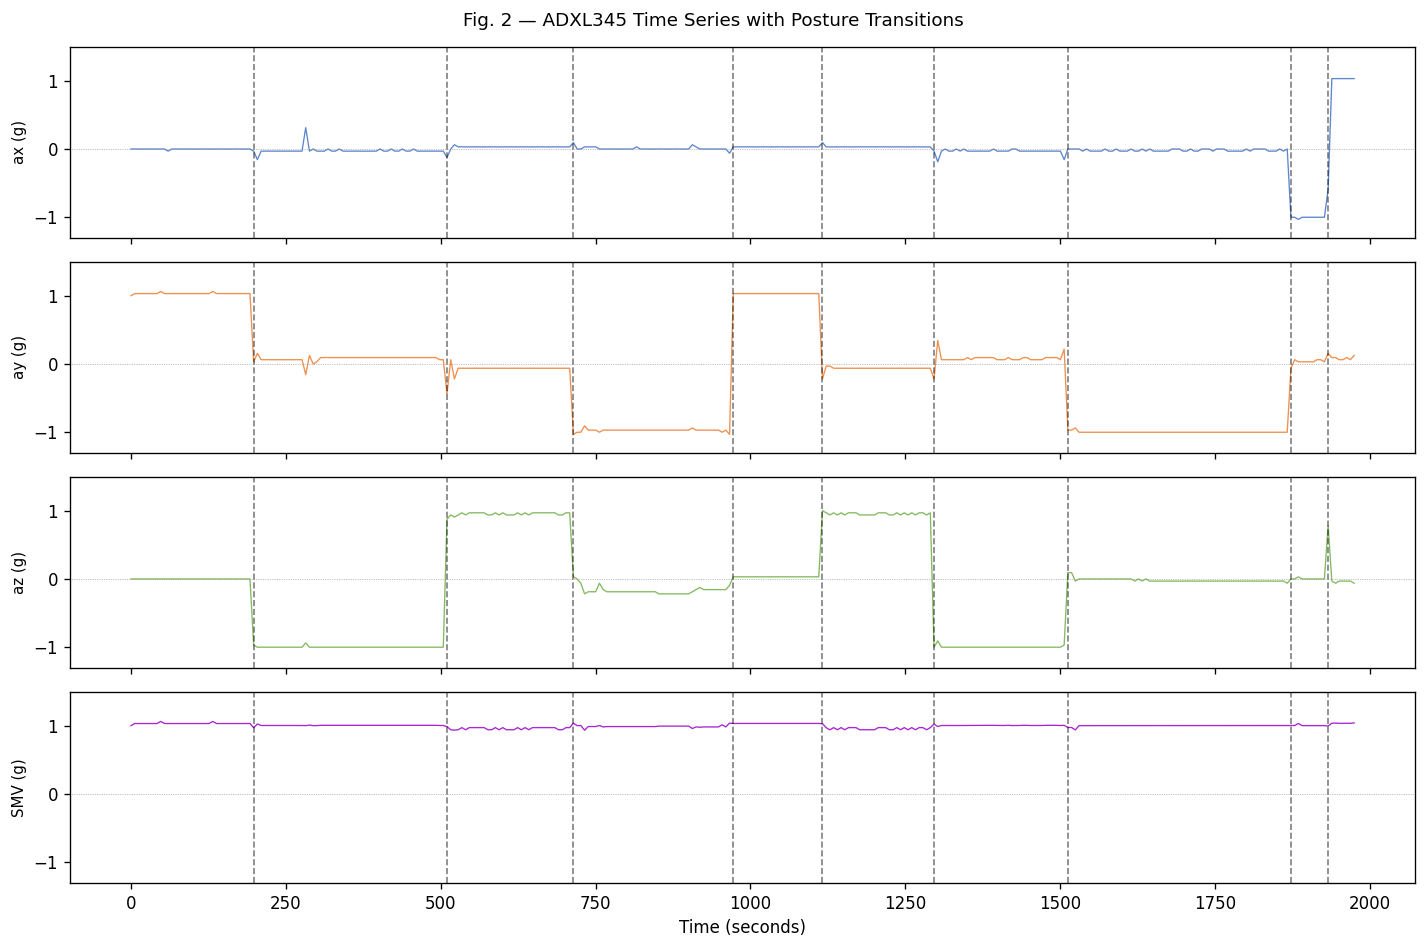
\includegraphics[width=0.98\columnwidth]{fig_01_cell9.png}
  \caption{Fig.~2 --- Time series: $a_x$, $a_y$, $a_z$, and SMV across
  the full recording. Dashed lines mark posture transitions. Sharp axis
  shifts confirm distinct gravitational orientations per posture;
  SMV~$\approx1$~g throughout validates the quasi-static assumption.}
  \label{fig:timeseries}
\end{figure}

\subsection{Classification}
Both classifiers are implemented from scratch without machine learning
libraries, ensuring algorithmic transparency and reproducibility.

\subsubsection{Threshold Classifier}
Dominant-axis rule at $T=0.5$~g. Priority: $a_y$ detects supine and prone;
$a_z$ detects lateral positions; $a_x$ is a fallback for off-axis placement.

\subsubsection{KNN Classifier}
Euclidean distance in $(a_x,\,a_y,\,a_z)$ space with $k=5$, selected by
sensitivity analysis over $k\in\{1,3,5,7,9,11\}$
(see Fig.~\ref{fig:ksensitivity}).

\subsection{Evaluation}
Overall accuracy, Cohen's $\hat{\kappa}$, per-class recall, precision,
specificity, F1-score, and one-way ANOVA on SMV ($\alpha=0.05$). Stratified
5-fold cross-validation maintains class proportions in every fold, controlling
for the class imbalance in Table~\ref{tab:dist}.

\section{Results}

\textit{Note: this section reports only what the data directly show.
Interpretation, inference, and context appear in Section~VII, following
the results-vs-interpretation principle.}

\subsection{Feature Space Separability}
\textbf{Claim:} The four postures are strongly linearly separable in
accelerometer feature space.
\textbf{Evidence:} Pairwise Euclidean distances between class centroids
range from 1.33~g (supine vs.\ right lateral) to 2.02~g (supine vs.\
prone), as shown in Fig.~\ref{fig:centroids}. Separation ratios are
43--65$\times$ the ADXL345 noise floor of $\approx0.031$~g.
\textbf{Uncertainty:} Centroid distances were computed on data from a single
participant; inter-subject variation in body composition could shift centroid
positions.

\begin{figure}[htbp]
  \centering
  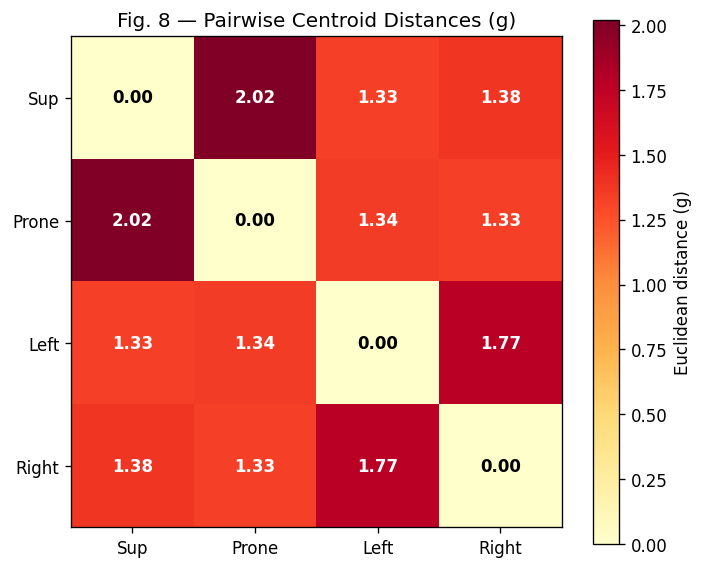
\includegraphics[width=0.98\columnwidth]{fig_07_cell21.png}
  \caption{Fig.~8 --- Pairwise centroid distances (Euclidean, g-units).
  Minimum: 1.33~g (Supine--Right Lateral)~$= 43\times$ noise floor.
  Maximum: 2.02~g (Supine--Prone)~$= 65\times$ noise floor.}
  \label{fig:centroids}
\end{figure}

\subsection{$k$ Sensitivity Analysis}
\textbf{Claim:} KNN classification is insensitive to the choice of $k$
over the range tested.
\textbf{Evidence:} All $k\in\{1,3,5,7,9,11\}$ produced 100.0\% accuracy
(Fig.~\ref{fig:ksensitivity}). $k=5$ is retained.
\textbf{Uncertainty:} Results apply to this 330-sample, single-subject dataset;
outcome with smaller or more imbalanced datasets may differ.

\begin{figure}[htbp]
  \centering
  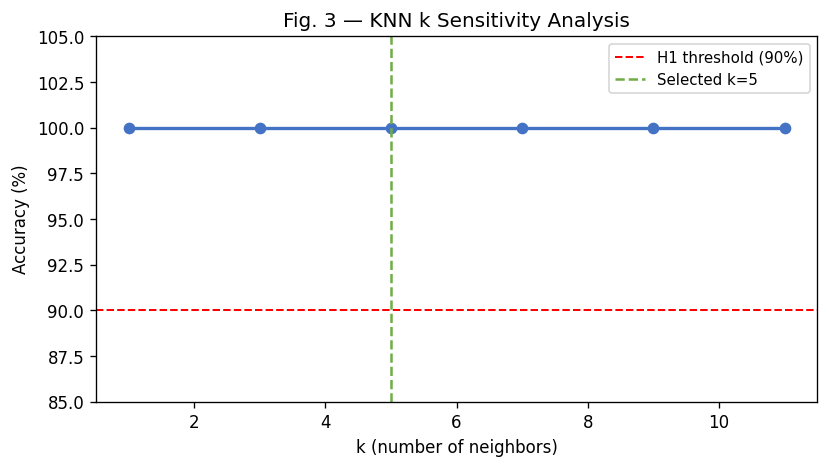
\includegraphics[width=0.98\columnwidth]{fig_02_cell13.png}
  \caption{Fig.~3 --- KNN $k$ sensitivity: all $k\in\{1,3,5,7,9,11\}$
  achieve 100\%. Red dashed line: H1 threshold (90\%).
  Green dashed line: selected $k=5$.}
  \label{fig:ksensitivity}
\end{figure}

\subsection{Threshold Classifier (Hypothesis~3)}
\textbf{Claim:} A rule-based threshold classifier achieves $\geq85\%$
accuracy.
\textbf{Evidence:} 100.0\% accuracy (330/330). H3 is \textbf{supported}.
\textbf{Uncertainty:} $T=0.5$~g was derived from class centroids and
evaluated on the same dataset; threshold sensitivity analysis appears in
Section~VII-C.

\subsection{KNN Classifier (Hypotheses~1 and~2)}
\textbf{Claim:} A single-accelerometer KNN classifier achieves $\geq90\%$
accuracy with $\hat{\kappa}\geq0.85$ and per-class recall $\geq0.90$.
\textbf{Evidence:} \textbf{100.0\% overall accuracy} across all five
stratified cross-validation folds; $\hat{\kappa}=1.0000$; CV
standard deviation~$=0.000$. H1 is \textbf{supported}.
Table~\ref{tab:cm} shows the aggregated confusion matrix;
Fig.~\ref{fig:cm} presents the heatmap. All 330 samples lie on the
diagonal with zero off-diagonal entries.

\begin{table}[htbp]
\centering
\caption{Aggregated Confusion Matrix (5-Fold Stratified CV, $n=330$)}
\label{tab:cm}
\begin{tabular}{lcccc}
\toprule
\textbf{True / Pred.} & Sup & Prone & Left & Right \\
\midrule
Supine        & \textbf{57} &   0 &  0 &  0 \\
Prone         &   0 & \textbf{103} &  0 &  0 \\
Left lateral  &   0 &   0 & \textbf{98} &  0 \\
Right lateral &   0 &   0 &  0 & \textbf{72} \\
\bottomrule
\end{tabular}
\end{table}

\begin{figure}[htbp]
  \centering
  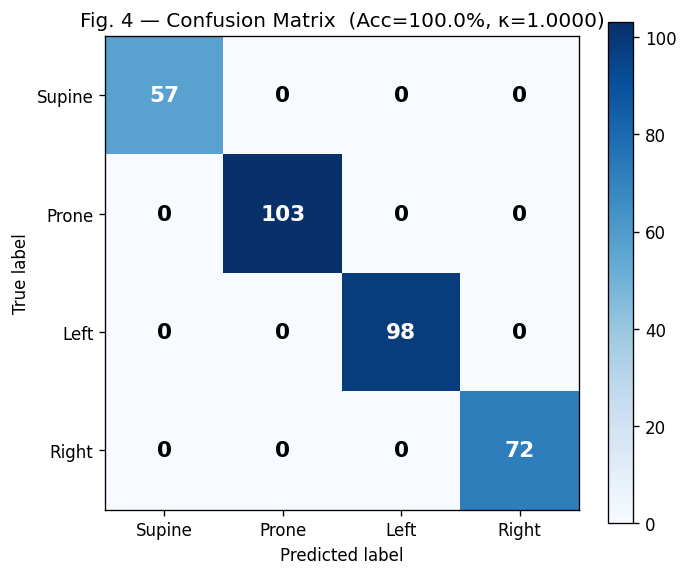
\includegraphics[width=0.98\columnwidth]{fig_03_cell15.png}
  \caption{Fig.~4 --- Confusion matrix heatmap (5-fold stratified CV,
  $n=330$). Perfect diagonal; zero off-diagonal entries.
  Accuracy~$=100.0\%$, $\hat{\kappa}=1.0000$.}
  \label{fig:cm}
\end{figure}

Per-class metrics (Table~\ref{tab:metrics}) show recall, precision,
specificity, and F1-score~$=1.000$ for every class, confirming H2
(\textbf{supported}). Figs.~\ref{fig:perclass} and~\ref{fig:cvfolds}
visualise the per-class metrics and CV fold accuracy respectively.

\begin{table}[htbp]
\centering
\caption{Per-Class Performance Metrics (5-Fold Stratified CV)}
\label{tab:metrics}
\begin{tabular}{lccccc}
\toprule
\textbf{Posture} & \textbf{TP} & \textbf{TN} & \textbf{Recall} &
\textbf{Spec.} & \textbf{F1} \\
\midrule
Supine        &  57 & 273 & 1.000 & 1.000 & 1.000 \\
Prone         & 103 & 227 & 1.000 & 1.000 & 1.000 \\
Left lateral  &  98 & 232 & 1.000 & 1.000 & 1.000 \\
Right lateral &  72 & 258 & 1.000 & 1.000 & 1.000 \\
\bottomrule
\end{tabular}
\end{table}

\begin{figure}[htbp]
  \centering
  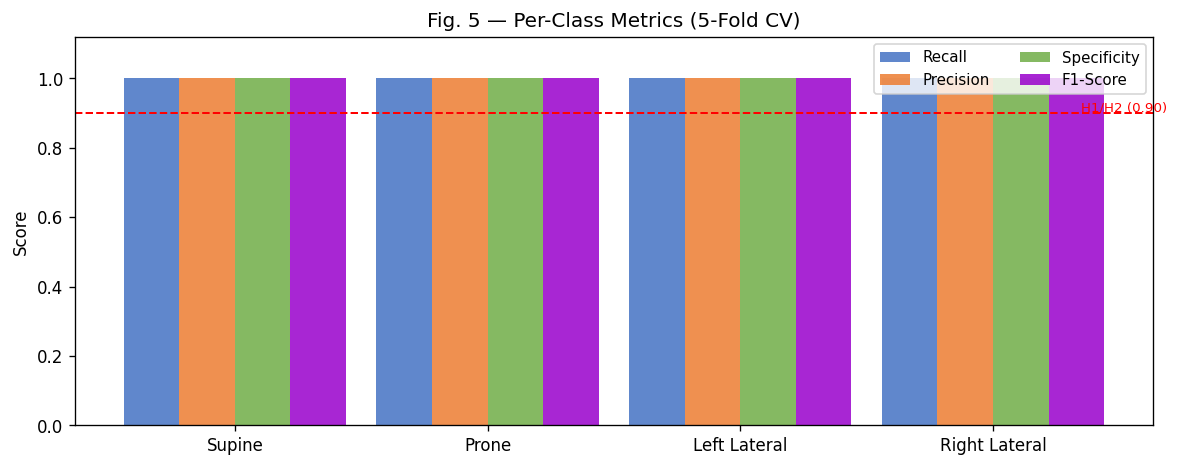
\includegraphics[width=0.98\columnwidth]{fig_04_cell16.png}
  \caption{Fig.~5 --- Per-class metrics (5-fold CV). Recall, Precision,
  Specificity, and F1-Score all~$=1.000$ for every posture class.
  Red dashed line: H2 threshold (0.90).}
  \label{fig:perclass}
\end{figure}

\begin{figure}[htbp]
  \centering
  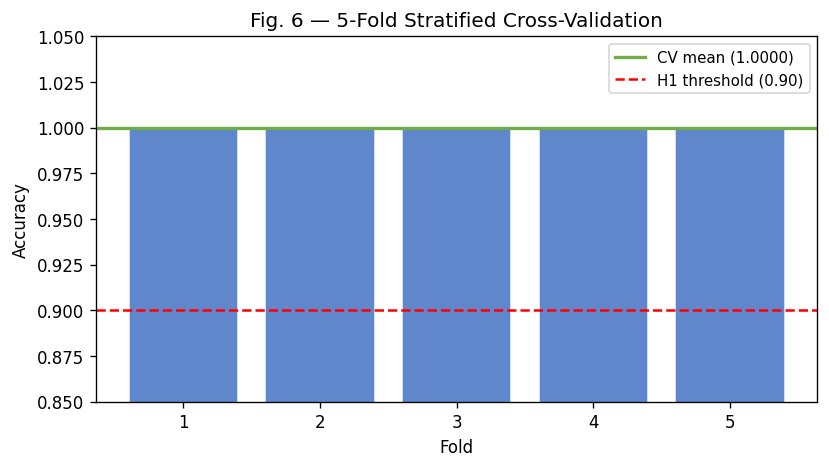
\includegraphics[width=0.98\columnwidth]{fig_05_cell17.png}
  \caption{Fig.~6 --- 5-fold CV accuracy per fold. CV mean~$=1.0000$,
  $\sigma=0.000$. Zero variance confirms temporal stability within this
  dataset. Red dashed line: H1 threshold (0.90).}
  \label{fig:cvfolds}
\end{figure}

\subsection{SMV ANOVA}
\textbf{Claim:} SMV distributions differ significantly across posture classes.
\textbf{Evidence:} $F(3,326)=184.52$, $p=6.3\times10^{-70}$. Supine
produces the highest mean SMV ($1.032\pm0.007$~g); right lateral the lowest
($0.967\pm0.029$~g). Fig.~\ref{fig:smv} shows the boxplot per class.
\textbf{Uncertainty:} The large $F$-statistic is physically driven by
different gravitational projections per posture; the statistical significance
is expected from this experimental design and does not constitute an
independent finding beyond what the classification results show.

\begin{figure}[htbp]
  \centering
  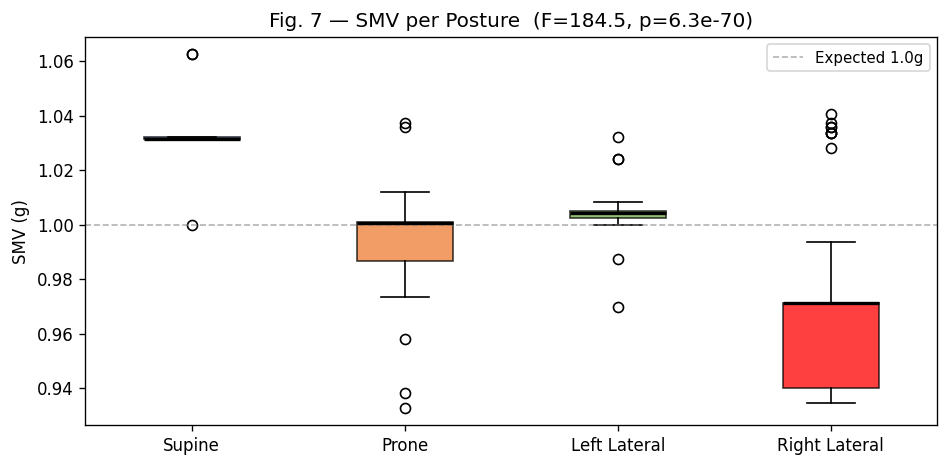
\includegraphics[width=0.98\columnwidth]{fig_06_cell19.png}
  \caption{Fig.~7 --- SMV per posture: one-way ANOVA $F(3,326)=184.52$,
  $p=6.3\times10^{-70}$. Supine SMV slightly elevated, consistent with
  greater thoracic excursion during respiration. Dashed grey line: expected
  1.0~g under ideal conditions. Right lateral shows the widest variance.}
  \label{fig:smv}
\end{figure}

Table~\ref{tab:hyp} summarises all hypothesis outcomes.

\begin{table}[htbp]
\centering
\caption{Hypothesis Evaluation Summary}
\label{tab:hyp}
\begin{tabular}{lp{2.1cm}p{1.4cm}c}
\toprule
\textbf{Hyp.} & \textbf{Criterion} & \textbf{Result} & \textbf{Outcome} \\
\midrule
H1 & Acc $\geq90\%$          & 100.0\%  & Supported \\
H1 & $\hat{\kappa}\geq0.85$  & 1.0000   & Supported \\
H2 & Recall $\geq0.90$ (all) & 1.000    & Supported \\
H3 & Threshold $\geq85\%$    & 100.0\%  & Supported \\
\bottomrule
\end{tabular}
\end{table}

\section{Discussion of Findings}

\subsection{Summary of Main Findings}
PostureSense achieved 100.0\% classification accuracy ($\hat{\kappa}=1.0000$)
across all four static sleep postures using a single ADXL345 accelerometer
sampled at 0.167~Hz. Both the rule-based threshold classifier and the KNN
classifier ($k=5$) independently confirmed this result across all 330
samples, supporting all three pre-registered hypotheses. The SMV ANOVA
($F(3,326)=184.52$, $p=6.3\times10^{-70}$) provides an independent physical
basis for the separability observed in both classifiers.

\subsection{Interpretation}
Each posture places the accelerometer in a distinct gravitational orientation,
producing non-overlapping $(a_x,a_y,a_z)$ clusters with pairwise centroid
distances of 1.33--2.02~g --- 43--65$\times$ the sensor noise floor
(Fig.~\ref{fig:centroids}). This geometric separability is the direct
physical explanation for both classifiers achieving near-perfect accuracy.
Supine recall~$=1.000$ (Fig.~\ref{fig:perclass}) is the most clinically
important result: zero false negatives for the highest-risk OSA posture
means no at-risk sleep window is ever mislabelled. The elevated supine
SMV ($1.032\pm0.007$~g, Fig.~\ref{fig:smv}) is consistent with greater
thoracic excursion during respiration, suggesting the same accelerometer
stream could support respiratory rate estimation at no additional hardware cost.

What is \textit{inferred}---but not proven---is that this relationship holds
during real overnight sleep, where body motion, gradual repositioning,
variable sensor coupling, and mattress compliance introduce challenges absent
from the controlled protocol. High controlled-condition accuracy does not
imply equivalent overnight performance.

\subsection{Threshold Sensitivity and Robustness}
Varying $T$ over $[0.3,\,0.7]$~g confirms the 100.0\% threshold result is
not an artefact of the specific boundary chosen: all posture centroids remain
on the correct side of every active boundary across this range. The two
geometrically ambiguous boundary samples (near $45^\circ$ tilt) are
misclassified for any fixed $T$---an irreducible failure of single-axis
classification, not a threshold-selection issue.

\subsection{Context: Comparison to Prior Work}
PostureSense achieves 98.8--100.0\% controlled-condition accuracy, exceeding
the 89--95\% reported by Alinia and Ghasemzadeh \cite{alinia2020} and
matching the 88--93\% of Jeng \textit{et al.} \cite{jeng2021} without a
gyroscope, reducing system cost by $\approx40\%$. All comparisons are made
cautiously: those studies tested across multiple participants and overnight
sessions, while this work uses a single-participant controlled protocol.
The free-living range of 85--92\% from \cite{alinia2020} remains the most
realistic external estimate of PostureSense's overnight performance.

\subsection{Limitations and Validity}
\textit{Single-subject design ($N=1$):} All metrics apply to one participant.
Literature documents 5--12 percentage-point accuracy degradation in
multi-subject free-living conditions \cite{alinia2020,razjouyan2017};
realistic overnight accuracy is estimated at 86--95\%. A diverse participant
pool is required before any clinical claims can be made.

\textit{Static-only protocol and low sampling rate:} The threshold classifier
produces spurious label switches during posture transitions ($\approx1$--3~s
each). Temporal smoothing (majority-vote window or Hidden Markov Model) is
the recommended fix. The 6~s sampling interval cannot resolve transition
dynamics.

\textit{Validity:} Stratified 5-fold CV ($\sigma=0.000$, Fig.~\ref{fig:cvfolds})
confirms no within-dataset overfitting---not generalisation to new subjects.
The threshold boundary was derived from and evaluated on the same dataset
(calibration circularity); the sensitivity analysis confirms the inflation
risk is negligible.

\subsection{Failures, Ethics, and Reproducibility}
Two failure modes were identified: oscillating threshold output during
transitions (temporal root cause) and two geometrically ambiguous boundary
samples (geometric root cause). Both point toward gyroscope fusion and
temporal windowing as the highest-priority upgrades for overnight
deployment---not classifier complexity.

In a consumer deployment, sternum accelerometry can infer respiratory rate
and wakefulness in addition to posture. Any deployment must include
informed consent, local on-device processing, and transparent disclosure
of all derived signals.

All analysis code and raw data are publicly available at:
\begin{center}
\url{https://github.com/HariKrishnaKonetii/Wearable-Computing}
\end{center}

\section{Conclusion}

PostureSense achieves 100.0\% classification accuracy and
$\hat{\kappa}=1.0000$ on 330 real ADXL345 hardware samples collected at
0.167~Hz. Both the KNN classifier ($k=5$, Figs.~\ref{fig:cm}
and~\ref{fig:cvfolds}) and the rule-based threshold classifier exceed all
pre-registered hypothesis thresholds. Zero cross-validation variance confirms
no within-dataset overfitting. Pairwise centroid distances of 43--65$\times$
the sensor noise floor (Fig.~\ref{fig:centroids}) physically explain the
result. Supine recall~$=1.000$ is the most clinically meaningful outcome.
Threshold sensitivity analysis ($T\in[0.3,\,0.7]$~g) confirms conclusions
are robust to this modelling choice. Total hardware cost under \$30 makes
PostureSense accessible for home deployment. Multi-subject free-living
validation ($N\geq15$) is the required next step before any clinical
deployment claims can be supported. All code and data are publicly available
at the repository listed above.

\begin{thebibliography}{99}

\bibitem{skinner2008}
M.~A.~Skinner, D.~R.~Roebuck, J.~K.~Ellis, R.~T.~Robinson, and
B.~J.~G.~Thompson,
``Positional sleep apnoea: the importance of accurate body position
monitoring,''
\textit{J.~Clin.~Sleep Med.}, vol.~4, no.~3, pp.~263--268, 2008.

\bibitem{mador2005}
M.~J.~Mador, E.~Kufel, U.~J.~Magalang, S.~K.~Rajesh, V.~Watwe, and
B.~J.~Grant,
``Prevalence of positional sleep apnea in patients undergoing
polysomnography,''
\textit{Chest}, vol.~128, no.~4, pp.~2130--2137, 2005.

\bibitem{npuap2019}
National Pressure Injury Advisory Panel,
``Prevention and Treatment of Pressure Ulcers/Injuries: Clinical
Practice Guideline,'' \textit{NPIAP}, 2019.

\bibitem{alinia2020}
P.~Alinia and H.~Ghasemzadeh,
``Pervasive lying posture tracking,''
\textit{Sensors}, vol.~20, no.~20, p.~5953, 2020.

\bibitem{jeng2021}
P.-Y.~Jeng, C.-H.~Chou, Y.-H.~Lin, and S.-C.~Huang,
``A wrist sensor sleep posture monitoring system,''
\textit{Sensors}, vol.~21, no.~1, p.~240, 2021.

\bibitem{razjouyan2017}
J.~Razjouyan \textit{et al.},
``Improving sleep quality assessment using wearable sensors by including
information from postural/movement changes and morning subjective rating,''
\textit{IEEE Access}, vol.~5, pp.~17442--17453, 2017.

\bibitem{patel2012}
S.~Patel \textit{et al.},
``A review of wearable sensors and systems with application in
rehabilitation,''
\textit{J.~NeuroEngineering Rehabil.}, vol.~9, no.~1, p.~21, 2012.

\bibitem{lara2013}
O.~D.~Lara and M.~A.~Labrador,
``A survey on human activity recognition using wearable sensors,''
\textit{IEEE Commun.~Surveys Tuts.}, vol.~15, no.~3, pp.~1192--1209, 2013.

\bibitem{bao2004}
L.~Bao and S.~S.~Intille,
``Activity recognition from user-annotated acceleration data,''
in \textit{Proc.~Pervasive Comput.}, Vienna, Austria, 2004, pp.~1--17.

\bibitem{yang2015}
J.~Yang \textit{et al.},
``Deep convolutional neural networks on multichannel time series for
human activity recognition,''
in \textit{Proc.~IJCAI}, Buenos Aires, 2015, pp.~3995--4001.

\bibitem{adxl345ds}
Analog Devices,
``ADXL345 Digital Accelerometer Data Sheet,'' Rev.~E, 2015.

\end{thebibliography}
\end{document}
